% Figura cuerpo B2 (3.3.5): las tres ecuaciones como sistema: quién decide qué y por qué se resuelve hacia adelante
\documentclass[tikz,border=3pt]{standalone}
\usepackage[T1]{fontenc}
\usepackage[utf8]{inputenc}
\usepackage{amsmath}
\usepackage{amssymb}
\usetikzlibrary{arrows.meta,calc,positioning}
\begin{document}
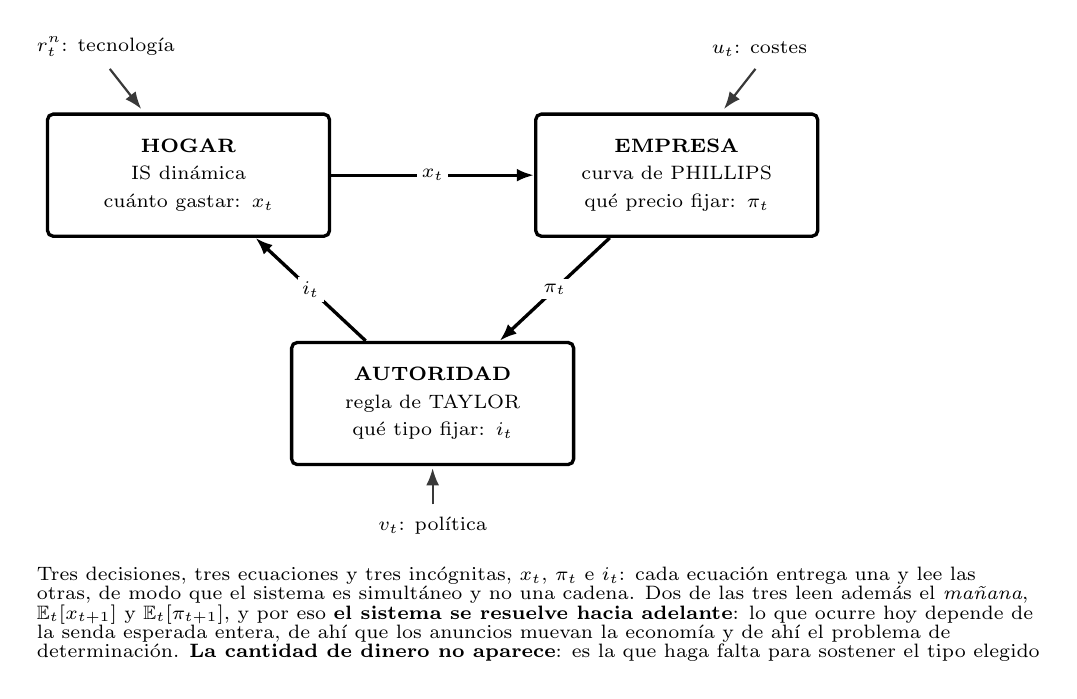
\begin{tikzpicture}[>={Latex[length=2.2mm]}, font=\scriptsize,
  caja/.style={draw, very thick, rounded corners=2pt, align=center, inner sep=4pt, text width=3.3cm, minimum height=1.55cm, font=\scriptsize},
  fl/.style={->, very thick},
  rot/.style={midway, fill=white, inner sep=1.6pt, font=\scriptsize},
  ex/.style={->, thick, gray!45!black}]

  \node[caja] (H) at (0,2.9)   {\textbf{HOGAR}\\[2pt]IS dinámica\\[2pt]cuánto gastar: $x_{t}$};
  \node[caja] (E) at (6.2,2.9) {\textbf{EMPRESA}\\[2pt]curva de PHILLIPS\\[2pt]qué precio fijar: $\pi_{t}$};
  \node[caja] (A) at (3.1,0)   {\textbf{AUTORIDAD}\\[2pt]regla de TAYLOR\\[2pt]qué tipo fijar: $i_{t}$};

  \draw[fl] (H) -- node[rot]{$x_{t}$} (E);
  \draw[fl] (E) -- node[rot]{$\pi_{t}$} (A);
  \draw[fl] (A) -- node[rot]{$i_{t}$} (H);

  \draw[ex] (-1.0,4.25) -- (-0.60,3.74);
  \node[anchor=south, font=\scriptsize] at (-1.05,4.28) {$r^{n}_{t}$: tecnología};
  \draw[ex] (7.2,4.25) -- (6.80,3.74);
  \node[anchor=south, font=\scriptsize] at (7.25,4.28) {$u_{t}$: costes};
  \draw[ex] (3.1,-1.28) -- (3.1,-0.82);
  \node[anchor=north, font=\scriptsize] at (3.1,-1.32) {$v_{t}$: política};

  \node[align=left, anchor=north west, font=\scriptsize] at (-2.05,-1.95)
    {Tres decisiones, tres ecuaciones y tres incógnitas, $x_{t}$, $\pi_{t}$ e $i_{t}$: cada ecuación entrega una y lee las\\[-1pt]otras, de modo que el sistema es simultáneo y no una cadena. Dos de las tres leen además el \textit{mañana},\\[-1pt]$\mathbb{E}_{t}[x_{t+1}]$ y $\mathbb{E}_{t}[\pi_{t+1}]$, y por eso \textbf{el sistema se resuelve hacia adelante}: lo que ocurre hoy depende de\\[-1pt]la senda esperada entera, de ahí que los anuncios muevan la economía y de ahí el problema de\\[-1pt]determinación. \textbf{La cantidad de dinero no aparece}: es la que haga falta para sostener el tipo elegido};
\end{tikzpicture}
\end{document}
